\documentclass[12pt,a4paper]{article}
\usepackage{amsmath}
\usepackage{graphicx}
\usepackage{geometry}
\usepackage{float}
\geometry{left=2cm,right=2cm,top=2.5cm,bottom=2.5cm}

\title{\textbf{Kinematic and Singularity Analysis Report \\ with Explicit Matrix Operations}}
\author{Automated Generation System}
\date{\today}

\begin{document}
\maketitle

\section{Mathematical Formulation}
The closed-loop spatial kinematic constraint is given by:
\begin{equation}
    T_1(q_1) T_2(q_2) T_3(q_3) T_4(q_4) T_5(q_5) T_6(q_6) T_7(q_7) = I
\end{equation}
The velocity constraint yields $J_p \dot{\mathbf{q}}_p = - J_a \dot{q}_1$, where $J_p$ is the $6 \times 6$ passive Jacobian matrix obtained by removing the column corresponding to the driving joint $J_1$.

\section{Example Matrix Calculation at $q_1 = 0^\circ$}
The solved full joint configuration (in radians) is:
\begin{equation}
    \mathbf{q} = \begin{bmatrix} 0.0000 \\ 0.0010 \\ -0.0000 \\ -0.0020 \\ 0.0000 \\ -0.0010 \\ -0.0000 \end{bmatrix}
\end{equation}

Based on this configuration, the full $6 \times 7$ Jacobian matrix $J$ is evaluated as:
\begin{equation{
    \resizebox{0.95\textwidth}{!}{$ J = \begin{bmatrix}
  -0.000 & -0.000 & 0.000 & 2.500 & -0.003 & -2.500 & 0.000 \\
  -0.000 & -1.000 & -0.000 & 3.000 & -0.000 & 2.000 & 0.000 \\
  0.000 & 0.000 & -3.000 & 0.003 & -0.500 & 0.003 & -2.000 \\
  0.000 & 0.000 & 0.000 & 0.001 & 0.000 & 0.001 & -0.000 \\
  0.000 & 0.000 & -1.000 & -0.000 & -1.000 & 0.000 & 1.000 \\
  1.000 & 1.000 & 0.000 & -1.000 & 0.000 & 1.000 & 0.000
\end{bmatrix} $}
\end{equation}

By extracting the columns corresponding to the passive joints, we form the passive Jacobian $J_p \in \mathbb{R}^{6 \times 6}$:
\begin{equation}
    \resizebox{0.85\textwidth}{!}{$ J_p = \begin{bmatrix}
  -0.000 & 0.000 & 2.500 & -0.003 & -2.500 & 0.000 \\
  -1.000 & -0.000 & 3.000 & -0.000 & 2.000 & 0.000 \\
  0.000 & -3.000 & 0.003 & -0.500 & 0.003 & -2.000 \\
  0.000 & 0.000 & 0.001 & 0.000 & 0.001 & -0.000 \\
  0.000 & -1.000 & -0.000 & -1.000 & 0.000 & 1.000 \\
  1.000 & 0.000 & -1.000 & 0.000 & 1.000 & 0.000
\end{bmatrix} $}
\end{equation}

Applying Singular Value Decomposition (SVD) on $J_p = U \Sigma V^T$, the decomposition yields $U$:
\begin{equation}
    \resizebox{0.85\textwidth}{!}{$ U = \begin{bmatrix}
  -0.667 & -0.004 & -0.641 & 0.000 & 0.380 & 0.000 \\
  -0.671 & 0.001 & 0.738 & -0.000 & 0.068 & 0.000 \\
  -0.002 & 0.990 & -0.004 & 0.142 & -0.000 & 0.000 \\
  -0.000 & 0.000 & 0.000 & 0.000 & 0.000 & -1.000 \\
  -0.000 & 0.142 & -0.001 & -0.990 & -0.000 & -0.000 \\
  0.324 & 0.002 & 0.210 & -0.000 & 0.923 & 0.000
\end{bmatrix} $}
\end{equation}

The singular values matrix $\Sigma$ (diagonal):
\begin{equation}
    \resizebox{0.85\textwidth}{!}{$ \Sigma = \begin{bmatrix}
  4.177 & 0.000 & 0.000 & 0.000 & 0.000 & 0.000 \\
  0.000 & 3.669 & 0.000 & 0.000 & 0.000 & 0.000 \\
  0.000 & 0.000 & 3.355 & 0.000 & 0.000 & 0.000 \\
  0.000 & 0.000 & 0.000 & 1.669 & 0.000 & 0.000 \\
  0.000 & 0.000 & 0.000 & 0.000 & 0.892 & 0.000 \\
  0.000 & 0.000 & 0.000 & 0.000 & 0.000 & 0.000
\end{bmatrix} $}
\end{equation}

And the transposed right singular vectors matrix $V^T$:
\begin{equation}
    \resizebox{0.85\textwidth}{!}{$ V^T = \begin{bmatrix}
  0.238 & 0.002 & -0.959 & 0.001 & 0.155 & 0.001 \\
  0.000 & -0.848 & -0.001 & -0.174 & 0.004 & -0.501 \\
  -0.157 & 0.003 & 0.119 & 0.001 & 0.980 & 0.002 \\
  -0.000 & 0.338 & 0.000 & 0.551 & -0.000 & -0.763 \\
  0.958 & 0.001 & 0.258 & -0.001 & 0.123 & -0.000 \\
  0.001 & -0.408 & 0.000 & 0.816 & -0.000 & 0.408
\end{bmatrix} $}
\end{equation}

\section{Analysis Results \& Curve Fitting}
\begin{figure}[H]
    \centering
    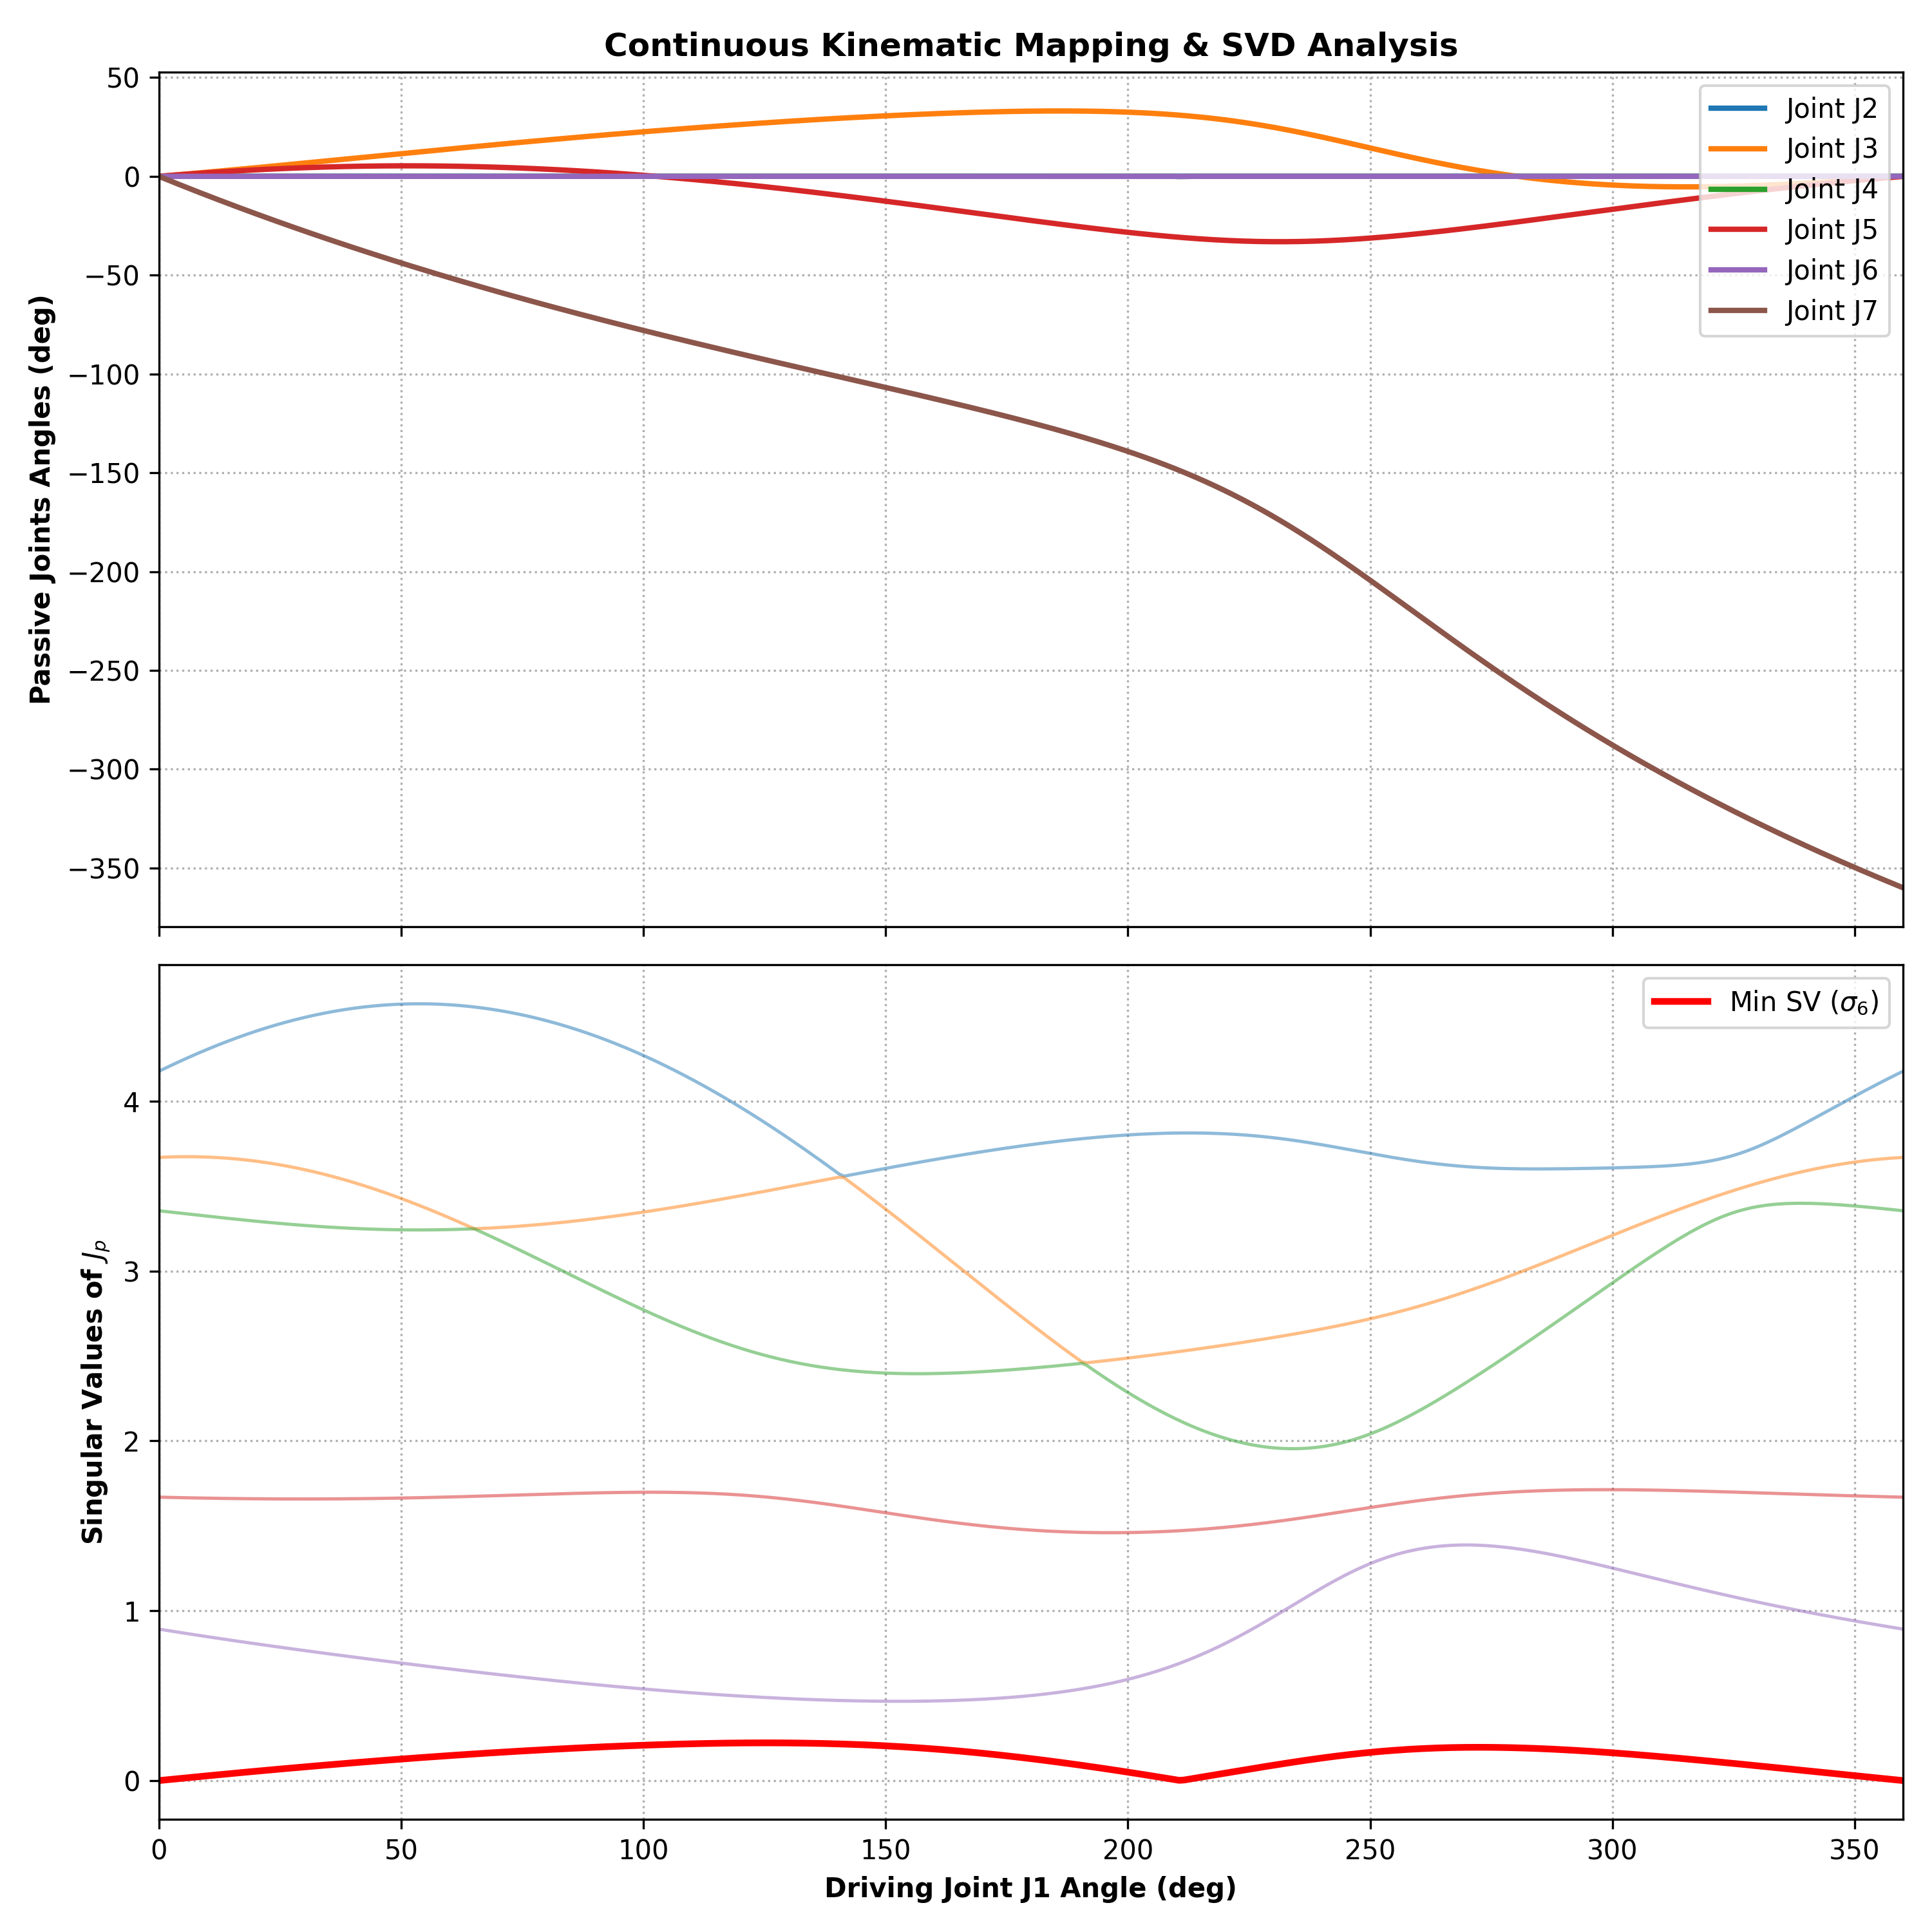
\includegraphics[width=0.9\textwidth]{j1_analysis_plot.png}
    \caption{Kinematic mapping and singular value evolution driven by $J_1$.}
\end{figure}

The empirical curve fitting formulas for the passive joints are derived as follows:
\begin{itemize}
\item \textbf{Joint J2:} \\ $Q_{J2}(x) = +0.000 -0.001\cos(x) -0.000\sin(x) +0.000\cos(2x) +0.001\sin(2x) -0.000\cos(3x) -0.001\sin(3x) -0.000\cos(4x) +0.001\sin(4x) +0.000\cos(5x) -0.000\sin(5x)$
\item \textbf{Joint J3:} \\ $Q_{J3}(x) = +14.741 -17.158\cos(x) +7.200\sin(x) +2.094\cos(2x) +3.424\sin(2x) +0.619\cos(3x) -0.949\sin(3x) -0.366\cos(4x) -0.023\sin(4x) +0.062\cos(5x) +0.112\sin(5x)$
\item \textbf{Joint J4:} \\ $Q_{J4}(x) = -0.000 +0.001\cos(x) +0.001\sin(x) -0.000\cos(2x) -0.001\sin(2x) +0.000\cos(3x) +0.001\sin(3x) +0.001\cos(4x) -0.001\sin(4x) -0.001\cos(5x) +0.000\sin(5x)$
\item \textbf{Joint J5:} \\ $Q_{J5}(x) = -11.728 +11.633\cos(x) +14.541\sin(x) +0.432\cos(2x) -1.922\sin(2x) -0.460\cos(3x) +0.224\sin(3x) +0.143\cos(4x) +0.068\sin(4x) -0.013\cos(5x) -0.053\sin(5x)$
\item \textbf{Joint J6:} \\ $Q_{J6}(x) = -0.000 +0.001\cos(x) +0.000\sin(x) -0.000\cos(2x) -0.001\sin(2x) +0.000\cos(3x) +0.001\sin(3x) +0.000\cos(4x) -0.001\sin(4x) -0.000\cos(5x) +0.000\sin(5x)$
\item \textbf{Joint J7:} \\ 
\textit{Model 1: 7th-order Polynomial} \\ 
$Q_{J7\text{-Poly}}(x) = -6.048020e-02x^{7} +1.278333e+00x^{6} -1.030244e+01x^{5} +3.982107e+01x^{4} -7.859981e+01x^{3} +8.140858e+01x^{2} -8.419649e+01x +2.276139e+00$ \\ 
\vspace{0.5em} \\ 
\textit{Model 2: 5th-order Fourier Series with Linear Trend} \\ 
$Q_{J7\text{-Fourier}}(x) = +26.400 -57.274x -28.791\cos(x) -7.297\sin(x) +1.662\cos(2x) +5.368\sin(2x) +1.079\cos(3x) -1.158\sin(3x) -0.509\cos(4x) -0.079\sin(4x) +0.074\cos(5x) +0.174\sin(5x)$
\end{itemize}
\end{document}
